% !TeX spellcheck = en_US
\textbf{14.10.2019}
\begin{itemize}
	\item Example:
	\begin{align*}
		e^{-20}=1-20+\frac{400}{2}-\frac{8000}{6}+..+-.. \frac{x^n}{n!}
	\end{align*}
	is problematic when you perform addition!
	\item Here comes the tableau
	\item IEEE 
	\begin{itemize}
		\item Standards: example: 754 (1985,2008,2018)
		\item Konverenz ARITH
		\item Institute of Electrical and Electronics Engineers
		\item Standard 1788 - for intervals/ interval arithmetic
	\end{itemize}
	\item Scientific Computation (step by step) %TODO make a node diagram later!
	\begin{enumerate}
		\item definition of problem
		\item \emph{simplification}
		\item physical problem
		\item \emph{model error}
		\item mathematical modeling
		\item \emph{approximation error}
		\item mathematical approximation
		\item \emph{rounding error}
		\item computation
		\item \emph{error analysis}
	\end{enumerate}
	So we have 4 possible sources of errors!
	\item numerical differentiation (derivatives)
	\begin{align*}
		f'(x)\approx \frac{f(x+h)-f(x-h)}{2h} \quad \text{ for small $h$}, h > 0
	\end{align*}
	With smaller $h$ we get better results, \emph{but} do not make $h$ to small. Then it is going to be even worse, because we get rounding - off error.
	\bigskip
	\textbf{15.10.2019}\\
	\item Scientific software in trouble\\
	\begin{tabularx}{\textwidth}{|X|X|X|}
		\hline
		\textbf{mathematics/brain}   & \textbf{app/software}    & \textbf{Hardware/Comp.} \\
		real, complex numbers & floating point numbers & FPN \\
		dense continuum & discrete grid & less fixed NFs\\
		strong structure & weak algebraic structure & arithemtic structure\\
		order relation (OR) $\le$ & OR $\le$ & directed rounding \\
		OR $\subseteq$ & OR $\subseteq$ & directed rounding \\
		intervals, sets & guaranteed inclusions & directed rounding\\
		function & function value inclusions & directed rounding\\
		math. notation & math. notation & machine code\\
		math. objects & data abstraction, OOP & memory management \\
		math. operations & operator overload & memory management\\
		sequential methods & parallelization & multicore/ M-processor\\
		\hline
	\end{tabularx}
	$\to$ \person{Willian Kahan} (``directed roundings'')
	\item Number formats (NFs)
	\begin{enumerate}
		\item single 32 bit
		\item double 64 bit
		\item extended 80 bit 
		\item quadruple 128 bit
	\end{enumerate}
	\item Rounding 
	\begin{center}
		\tikzset{every picture/.style={line width=0.75pt}} %set default line width to 0.75pt        
		
		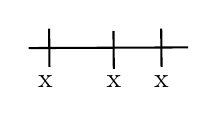
\begin{tikzpicture}[x=0.75pt,y=0.75pt,yscale=-1,xscale=1]
		%uncomment if require: \path (0,310); %set diagram left start at 0, and has height of 310
		
		%Straight Lines [id:da8610701323480399] 
		\draw    (46,41) -- (122.83,40.67) ;
		%Straight Lines [id:da4813505677920028] 
		\draw    (55.83,31.67) -- (56,50) ;
		%Straight Lines [id:da6888001065658323] 
		\draw    (109.83,31.67) -- (110,50) ;
		%Straight Lines [id:da482468059869271] 
		\draw    (86.83,32.67) -- (87,51) ;
		
		% Text Node
		\draw (87,57) node   [align=left] {x};
		% Text Node
		\draw (110,57) node   [align=left] {$\rndup$x};
		% Text Node
		\draw (54,57) node   [align=left] {$\rnddown$x};
		
		\end{tikzpicture}
	\end{center}
	Interval $X=(x,x) , \rndinterval X=[\rnddown x, \rndup x]$, but then we have errors in PC ($10^{20}+13)-10^{20} \to 10^{20}-10^{20} \to 0$ instead of 13 (Here rounding - off error is missing)
	\item Interval mathematics\\
	$\to$ \emph{Slogan}: Interval-algorithm always possible close and mathematical correct enclosures of solutions.\\
	If this is \emph{not} possible, errors must be reported!
	\begin{itemize}
		\item control rounding errors
		\item enclosure approximation errors
		\item enclosure of derivatives and remainders
		\item guaranteed enclosures of the solution (sets) 
		\item proof of existence of a solution in calculated interval
		\item If necessary, proof of  uniqueness of the solution
		\item control of step size, order, accuracy of results
		\item sharp termination condition and reliable error detection
		\item no fantasy solutions or numerical artifacts
	\end{itemize}
	Tools:
	\begin{itemize}
		\item automatic differentation
		\item LGS, NLGS
		\item Fixed-point theorems (e.g. \person{Brouwer})
		\item integration ,..
	\end{itemize}
	\item classic \person{Newton} method
	\newline $x_0=$ start value \smallskip
	\newline
	\begin{align*}
		x_k=x_{k-1}-\frac{f(x_{k-1})}{f'(x_{k-1})} \quad \with x_0 = \text{ initial value} 
	\end{align*}
	\item Interval \person{Newton} method
	\begin{align*}
		x_k=(mid(x_{k-1})-\frac{f(mid(x_{k-1})}{f'(x_{k-1})})\cap x_{k-1} \quad \with x_0 = \text{ initial interval} 
	\end{align*}
	(has quadratic convergence)
	\newline CISC $\to$ RISC $\to$ better pipelines (RISC is today in every processor!)
	\begin{align*}
		S_0=1+16^N-16^N+16^{N-1}\pm \dots +16^{-N}-16^{-N}+16^N-16^{N-1}+16^{N-1}-16^{N-1}
	\end{align*}
	calculation with 4 pipelines 
	% TODO (Here the drawing is missing)
	we have here obliteration problems!
	\item \person{Knuth} - computer science pioneer, \person{Turing}, \person{Wilkinson} 
	\item Requirements for programming systems
	\begin{itemize}
		\item mathematical notation (simple program structure, clear, reusable, modulary, overloading, simple formulas)
		\item Data abstraction (new data objects/ operations from existing operators combining
		\item automatic memory management (dynamic objects variable size)
		\item accuracy and inclusion
	\end{itemize}
\end{itemize}